%% bare_conf_compsoc.tex
%% V1.4b
%% 2015/08/26
%% by Michael Shell
%% See:
%% http://www.michaelshell.org/
%% for current contact information.
%%
%% This is a skeleton file demonstrating the use of IEEEtran.cls
%% (requires IEEEtran.cls version 1.8b or later) with an IEEE Computer
%% Society conference paper.
%%
%% Support sites:
%% http://www.michaelshell.org/tex/ieeetran/
%% http://www.ctan.org/pkg/ieeetran
%% and
%% http://www.ieee.org/

%%*************************************************************************
%% Legal Notice:
%% This code is offered as-is without any warranty either expressed or
%% implied; without even the implied warranty of MERCHANTABILITY or
%% FITNESS FOR A PARTICULAR PURPOSE! 
%% User assumes all risk.
%% In no event shall the IEEE or any contributor to this code be liable for
%% any damages or losses, including, but not limited to, incidental,
%% consequential, or any other damages, resulting from the use or misuse
%% of any information contained here.
%%
%% All comments are the opinions of their respective authors and are not
%% necessarily endorsed by the IEEE.
%%
%% This work is distributed under the LaTeX Project Public License (LPPL)
%% ( http://www.latex-project.org/ ) version 1.3, and may be freely used,
%% distributed and modified. A copy of the LPPL, version 1.3, is included
%% in the base LaTeX documentation of all distributions of LaTeX released
%% 2003/12/01 or later.
%% Retain all contribution notices and credits.
%% ** Modified files should be clearly indicated as such, including  **
%% ** renaming them and changing author support contact information. **
%%*************************************************************************


% *** Authors should verify (and, if needed, correct) their LaTeX system  ***
% *** with the testflow diagnostic prior to trusting their LaTeX platform ***
% *** with production work. The IEEE's font choices and paper sizes can   ***
% *** trigger bugs that do not appear when using other class files.       ***                          ***
% The testflow support page is at:
% http://www.michaelshell.org/tex/testflow/



\documentclass[conference,compsoc]{IEEEtran}
% Some/most Computer Society conferences require the compsoc mode option,
% but others may want the standard conference format.
%
% If IEEEtran.cls has not been installed into the LaTeX system files,
% manually specify the path to it like:
% \documentclass[conference,compsoc]{../sty/IEEEtran}





% Some very useful LaTeX packages include:
% (uncomment the ones you want to load)


% *** MISC UTILITY PACKAGES ***
%
\usepackage{ifpdf}
% Heiko Oberdiek's ifpdf.sty is very useful if you need conditional
% compilation based on whether the output is pdf or dvi.
% usage:
% \ifpdf
%   % pdf code
% \else
%   % dvi code
% \fi
% The latest version of ifpdf.sty can be obtained from:
% http://www.ctan.org/pkg/ifpdf
% Also, note that IEEEtran.cls V1.7 and later provides a builtin
% \ifCLASSINFOpdf conditional that works the same way.
% When switching from latex to pdflatex and vice-versa, the compiler may
% have to be run twice to clear warning/error messages.






% *** CITATION PACKAGES ***
%
\ifCLASSOPTIONcompsoc
  % IEEE Computer Society needs nocompress option
  % requires cite.sty v4.0 or later (November 2003)
  \usepackage[nocompress]{cite}
\else
  % normal IEEE
  \usepackage{cite}
\fi
% cite.sty was written by Donald Arseneau
% V1.6 and later of IEEEtran pre-defines the format of the cite.sty package
% \cite{} output to follow that of the IEEE. Loading the cite package will
% result in citation numbers being automatically sorted and properly
% "compressed/ranged". e.g., [1], [9], [2], [7], [5], [6] without using
% cite.sty will become [1], [2], [5]--[7], [9] using cite.sty. cite.sty's
% \cite will automatically add leading space, if needed. Use cite.sty's
% noadjust option (cite.sty V3.8 and later) if you want to turn this off
% such as if a citation ever needs to be enclosed in parenthesis.
% cite.sty is already installed on most LaTeX systems. Be sure and use
% version 5.0 (2009-03-20) and later if using hyperref.sty.
% The latest version can be obtained at:
% http://www.ctan.org/pkg/cite
% The documentation is contained in the cite.sty file itself.
%
% Note that some packages require special options to format as the Computer
% Society requires. In particular, Computer Society  papers do not use
% compressed citation ranges as is done in typical IEEE papers
% (e.g., [1]-[4]). Instead, they list every citation separately in order
% (e.g., [1], [2], [3], [4]). To get the latter we need to load the cite
% package with the nocompress option which is supported by cite.sty v4.0
% and later.





% *** GRAPHICS RELATED PACKAGES ***
%
\ifCLASSINFOpdf
  % \usepackage[pdftex]{graphicx}
  % declare the path(s) where your graphic files are
  % \graphicspath{{../pdf/}{../jpeg/}}
  % and their extensions so you won't have to specify these with
  % every instance of \includegraphics
  % \DeclareGraphicsExtensions{.pdf,.jpeg,.png}
\else
  % or other class option (dvipsone, dvipdf, if not using dvips). graphicx
  % will default to the driver specified in the system graphics.cfg if no
  % driver is specified.
  % \usepackage[dvips]{graphicx}
  % declare the path(s) where your graphic files are
  % \graphicspath{{../eps/}}
  % and their extensions so you won't have to specify these with
  % every instance of \includegraphics
  % \DeclareGraphicsExtensions{.eps}
\fi
% graphicx was written by David Carlisle and Sebastian Rahtz. It is
% required if you want graphics, photos, etc. graphicx.sty is already
% installed on most LaTeX systems. The latest version and documentation
% can be obtained at: 
% http://www.ctan.org/pkg/graphicx
% Another good source of documentation is "Using Imported Graphics in
% LaTeX2e" by Keith Reckdahl which can be found at:
% http://www.ctan.org/pkg/epslatex
%
% latex, and pdflatex in dvi mode, support graphics in encapsulated
% postscript (.eps) format. pdflatex in pdf mode supports graphics
% in .pdf, .jpeg, .png and .mps (metapost) formats. Users should ensure
% that all non-photo figures use a vector format (.eps, .pdf, .mps) and
% not a bitmapped formats (.jpeg, .png). The IEEE frowns on bitmapped formats
% which can result in "jaggedy"/blurry rendering of lines and letters as
% well as large increases in file sizes.
%
% You can find documentation about the pdfTeX application at:
% http://www.tug.org/applications/pdftex





% *** MATH PACKAGES ***
%
\usepackage{amsmath}
\usepackage{cuted}
% A popular package from the American Mathematical Society that provides
% many useful and powerful commands for dealing with mathematics.
%
% Note that the amsmath package sets \interdisplaylinepenalty to 10000
% thus preventing page breaks from occurring within multiline equations. Use:
%\interdisplaylinepenalty=2500
% after loading amsmath to restore such page breaks as IEEEtran.cls normally
% does. amsmath.sty is already installed on most LaTeX systems. The latest
% version and documentation can be obtained at:
% http://www.ctan.org/pkg/amsmath
\newcommand\numberthis{\addtocounter{equation}{1}\tag{\theequation}}




% *** SPECIALIZED LIST PACKAGES ***
%
\usepackage{algorithmic}
% algorithmic.sty was written by Peter Williams and Rogerio Brito.
% This package provides an algorithmic environment fo describing algorithms.
% You can use the algorithmic environment in-text or within a figure
% environment to provide for a floating algorithm. Do NOT use the algorithm
% floating environment provided by algorithm.sty (by the same authors) or
% algorithm2e.sty (by Christophe Fiorio) as the IEEE does not use dedicated
% algorithm float types and packages that provide these will not provide
% correct IEEE style captions. The latest version and documentation of
% algorithmic.sty can be obtained at:
% http://www.ctan.org/pkg/algorithms
% Also of interest may be the (relatively newer and more customizable)
% algorithmicx.sty package by Szasz Janos:
% http://www.ctan.org/pkg/algorithmicx




% *** ALIGNMENT PACKAGES ***
%
\usepackage{array}
% Frank Mittelbach's and David Carlisle's array.sty patches and improves
% the standard LaTeX2e array and tabular environments to provide better
% appearance and additional user controls. As the default LaTeX2e table
% generation code is lacking to the point of almost being broken with
% respect to the quality of the end results, all users are strongly
% advised to use an enhanced (at the very least that provided by array.sty)
% set of table tools. array.sty is already installed on most systems. The
% latest version and documentation can be obtained at:
% http://www.ctan.org/pkg/array


% IEEEtran contains the IEEEeqnarray family of commands that can be used to
% generate multiline equations as well as matrices, tables, etc., of high
% quality.




% *** SUBFIGURE PACKAGES ***
%\ifCLASSOPTIONcompsoc
%  \usepackage[caption=false,font=footnotesize,labelfont=sf,textfont=sf]{subfig}
%\else
%  \usepackage[caption=false,font=footnotesize]{subfig}
%\fi
% subfig.sty, written by Steven Douglas Cochran, is the modern replacement
% for subfigure.sty, the latter of which is no longer maintained and is
% incompatible with some LaTeX packages including fixltx2e. However,
% subfig.sty requires and automatically loads Axel Sommerfeldt's caption.sty
% which will override IEEEtran.cls' handling of captions and this will result
% in non-IEEE style figure/table captions. To prevent this problem, be sure
% and invoke subfig.sty's "caption=false" package option (available since
% subfig.sty version 1.3, 2005/06/28) as this is will preserve IEEEtran.cls
% handling of captions.
% Note that the Computer Society format requires a sans serif font rather
% than the serif font used in traditional IEEE formatting and thus the need
% to invoke different subfig.sty package options depending on whether
% compsoc mode has been enabled.
%
% The latest version and documentation of subfig.sty can be obtained at:
% http://www.ctan.org/pkg/subfig




% *** FLOAT PACKAGES ***
%
%\usepackage{fixltx2e}
% fixltx2e, the successor to the earlier fix2col.sty, was written by
% Frank Mittelbach and David Carlisle. This package corrects a few problems
% in the LaTeX2e kernel, the most notable of which is that in current
% LaTeX2e releases, the ordering of single and double column floats is not
% guaranteed to be preserved. Thus, an unpatched LaTeX2e can allow a
% single column figure to be placed prior to an earlier double column
% figure.
% Be aware that LaTeX2e kernels dated 2015 and later have fixltx2e.sty's
% corrections already built into the system in which case a warning will
% be issued if an attempt is made to load fixltx2e.sty as it is no longer
% needed.
% The latest version and documentation can be found at:
% http://www.ctan.org/pkg/fixltx2e


%\usepackage{stfloats}
% stfloats.sty was written by Sigitas Tolusis. This package gives LaTeX2e
% the ability to do double column floats at the bottom of the page as well
% as the top. (e.g., "\begin{figure*}[!b]" is not normally possible in
% LaTeX2e). It also provides a command:
%\fnbelowfloat
% to enable the placement of footnotes below bottom floats (the standard
% LaTeX2e kernel puts them above bottom floats). This is an invasive package
% which rewrites many portions of the LaTeX2e float routines. It may not work
% with other packages that modify the LaTeX2e float routines. The latest
% version and documentation can be obtained at:
% http://www.ctan.org/pkg/stfloats
% Do not use the stfloats baselinefloat ability as the IEEE does not allow
% \baselineskip to stretch. Authors submitting work to the IEEE should note
% that the IEEE rarely uses double column equations and that authors should try
% to avoid such use. Do not be tempted to use the cuted.sty or midfloat.sty
% packages (also by Sigitas Tolusis) as the IEEE does not format its papers in
% such ways.
% Do not attempt to use stfloats with fixltx2e as they are incompatible.
% Instead, use Morten Hogholm'a dblfloatfix which combines the features
% of both fixltx2e and stfloats:
%
% \usepackage{dblfloatfix}
% The latest version can be found at:
% http://www.ctan.org/pkg/dblfloatfix




% *** PDF, URL AND HYPERLINK PACKAGES ***
%
\usepackage{url}
% url.sty was written by Donald Arseneau. It provides better support for
% handling and breaking URLs. url.sty is already installed on most LaTeX
% systems. The latest version and documentation can be obtained at:
% http://www.ctan.org/pkg/url
% Basically, \url{my_url_here}.




% *** Do not adjust lengths that control margins, column widths, etc. ***
% *** Do not use packages that alter fonts (such as pslatex).         ***
% There should be no need to do such things with IEEEtran.cls V1.6 and later.
% (Unless specifically asked to do so by the journal or conference you plan
% to submit to, of course. )


% correct bad hyphenation here
\hyphenation{op-tical net-works semi-conduc-tor}


\begin{document}
%
% paper title
% Titles are generally capitalized except for words such as a, an, and, as,
% at, but, by, for, in, nor, of, on, or, the, to and up, which are usually
% not capitalized unless they are the first or last word of the title.
% Linebreaks \\ can be used within to get better formatting as desired.
% Do not put math or special symbols in the title.
\title{A Parallelism Oriented Three Phase Based Burst Buffering Aware Scheduler}


% author names and affiliations
% use a multiple column layout for up to three different
% affiliations
\author{\IEEEauthorblockN{Michael Shell}
\IEEEauthorblockA{School of Electrical and\\Computer Engineering\\
Georgia Institute of Technology\\
Atlanta, Georgia 30332--0250\\
Email: http://www.michaelshell.org/contact.html}
\and
\IEEEauthorblockN{Homer Simpson}
\IEEEauthorblockA{Twentieth Century Fox\\
Springfield, USA\\
Email: homer@thesimpsons.com}
\and
\IEEEauthorblockN{James Kirk\\ and Montgomery Scott}
\IEEEauthorblockA{Starfleet Academy\\
San Francisco, California 96678-2391\\
Telephone: (800) 555--1212\\
Fax: (888) 555--1212}}

% conference papers do not typically use \thanks and this command
% is locked out in conference mode. If really needed, such as for
% the acknowledgment of grants, issue a \IEEEoverridecommandlockouts
% after \documentclass

% for over three affiliations, or if they all won't fit within the width
% of the page (and note that there is less available width in this regard for
% compsoc conferences compared to traditional conferences), use this
% alternative format:
% 
%\author{\IEEEauthorblockN{Michael Shell\IEEEauthorrefmark{1},
%Homer Simpson\IEEEauthorrefmark{2},
%James Kirk\IEEEauthorrefmark{3}, 
%Montgomery Scott\IEEEauthorrefmark{3} and
%Eldon Tyrell\IEEEauthorrefmark{4}}
%\IEEEauthorblockA{\IEEEauthorrefmark{1}School of Electrical and Computer Engineering\\
%Georgia Institute of Technology,
%Atlanta, Georgia 30332--0250\\ Email: see http://www.michaelshell.org/contact.html}
%\IEEEauthorblockA{\IEEEauthorrefmark{2}Twentieth Century Fox, Springfield, USA\\
%Email: homer@thesimpsons.com}
%\IEEEauthorblockA{\IEEEauthorrefmark{3}Starfleet Academy, San Francisco, California 96678-2391\\
%Telephone: (800) 555--1212, Fax: (888) 555--1212}
%\IEEEauthorblockA{\IEEEauthorrefmark{4}Tyrell Inc., 123 Replicant Street, Los Angeles, California 90210--4321}}




% use for special paper notices
%\IEEEspecialpapernotice{(Invited Paper)}




% make the title area
\maketitle

% As a general rule, do not put math, special symbols or citations
% in the abstract
\begin{abstract}
In an computing world full of Big Data, moderate I/O performance drastically slows down the overall execution time of applications.
Burst buffer nodes comes to rescue by providing both higher bandwidth and IOPS.
In this paper, we model the execution of scientific applications that generates huge amount of data
on supercomputing system equipped with burst buffer nodes.
Computing nodes are then able to be freed earlier due to these efficient and reliable IO broker, 
possibly improving the utilization of task execution pipeline.
We thus characterize generic applications by 3 phases:
\textit{data stage in} phase, \textit{running} phase and \textit{data stage out} phase.
The novel 3-phase burst buffer aware workload scheduler is proposed on the assumption that
resources in different phases should be scheduled separately.
In both data stage input and output phase, it is possible to maximize data transfer throughput or task parallelism when allocating burst buffer.
In the running phase, we consider maximize the value of scheduling tasks with both computing node resources and burst buffer node demand.
Further investigating shows that all aforementioned optimization problems are equivalent to 0-1 knapsack problem,
requiring exponential time to solve.
We use dynamic programming and memorization technique to give precise solutions.
We simulate our 3 phase scheduler scheduling a supercomputing system in the scenarios 
both with and without burst buffer on a discrete event simulator to demonstrate that
1) burst buffer node can accelerate the execution pipeline of all task, 
thus improving the utilization of the computing nodes as well as task response time
2) our scheduling algorithm can further benefit burst buffer equipped system.
\end{abstract}

% no keywords

% For peer review papers, you can put extra information on the cover
% page as needed:
% \ifCLASSOPTIONpeerreview
% \begin{center} \bfseries EDICS Category: 3-BBND \end{center}
% \fi
%
% For peerreview papers, this IEEEtran command inserts a page break and
% creates the second title. It will be ignored for other modes.
\IEEEpeerreviewmaketitle

\section{Introduction}

%1. Current IO structure
In today's high-performance computing (HPC) systems,
application's performance is no longer only throttled by computation capability,
but also perceived I/O rate between
numerous amount of parallel processor cores and 
petabyte volume of storage equipments.
Current IO architects put IO forwarding nodes in charge of performing IO.
These IO gateways, together with parallel file system (PFS) software (client side),
sits between internal system networks that serving communication
between compute nodes and external system networks
that interconnects storage nodes\cite{Ross:IOSystem}.
Applications under this architecture can expect to achieve
810 GB/s per PFS sustained bandwidth in Trinity's Lustre\cite{TrinitySystem}
in later 2016, but still far from the target of 60 TB/s
for exa-scale computing platform\cite{Shalf:HPCCS:2010}.

%2. Challenge to current IO architecture and burst buffer come to resuce.
The challenge roots in the missing gap in HPC's memory hierarchy.
The ratio of IO rate of memory on the compute node to the storage disk
is 100 to 10,000 cycles\cite{TrinitySystem}.
Such a gap makes difference because scientific applications on HPC are exposed to
bursty IO patterns\cite{Carns:MSST:2011, Kim:PDSW:2010},
resulting from application's
defensive IO strategy\cite{Latham:CSD:2012, Naik:ICPPW:2009, Dennis:CUG:2009}
and the needs of subsequent processing of application output.


%On one hand, applications checkpoint periodically
%(so that computation could be restarted after system fault)
%or store intermediate output for subsequent analysis or visualization;
%on the other hand, pushing data from memory to external,
%parallel file system is unproductive due to the IO cycle gap.
%Though this conflict can be fixed by providing higher IO bandwidth capacity,
%another character of bursty IO pattern introduces another problem,
%underutilization of storage system.
%Production applications could generate hundreds of GB to
%tens of TB data in one IO request with significant idle interval.
%For example, observed idle interval of write-intensive jobs
%reported on Intrepid\cite{Liu:MSST:2012},
%varies from several minutes to 2 hours.

%3. Very high level intro to burst buffer
As an alternative storage design, burst buffer\cite{Bent:HBP:2011, Grider:EXA:2010}
is targeting on fixing the issues caused by bursty IO pattern.
It fills the gap in memory hierarchy with storage hardware technology
faster than traditional disks.
Bursty IO requests could thus be efficiently absorbed and spread out
into burst buffer nodes.
Researchers\cite{Liu:MSST:2012} have demonstrated that application perceived IO
bandwidth are significantly improved on burst buffer enabled system.
Given its usefulness, we expect user will explicitly request for
this new resource upon job submission.

%4. Our work, a new batch scheduler
In this paper, we propose Cerberus\footnote{In Greek mythology,
Cerberus is a monstrous multi-headed dog (3-phase scheduling scheme),
who guards the gates of the underworld to earth (HPC system),
preventing the dead (jobs) from leaving (running).},
a novel batch scheduler for HPC system with burst buffer awareness. 
We propose a 3-phase model for user job 
based on two of the most important usage cases of burst buffer: 
application checkpoint restart and data cache/pre-fetch for stage in/out. 
The lifetime of user job consists of \textit{stage in} phase, 
\textit{running} phase, and \textit{stage-out} phase. 
Unlike existing batch schedulers that 
make the permanent scheduling decision for job upon its submission, 
Cerberus re-evaluate job's requirement at each phase 
and make the optimal scheduling decisions respectively.

%5. The advantage of Cerberus.
Both the system and user job can benefit from Cerberus 3-phase scheduling.
System responsiveness can be greatly improved and
user jobs suffer less wait time. 
The burst buffer and compute nodes will be released right after the job enters next phase,
and become available to the following job.
Thus, the system utilization can be improved.
As Cerberus takes advantage of the parallelism of jobs in different phases,
system throughput also gets improved.

%6. Summarize our contribution
Our contributions in this paper are summarized as follows:

\begin{enumerate}
        \item Explore how HPC workload scheduler allocates burst buffer resources.
                We propose a 3-phase application model tailored the typical
                usage scenarios of burst buffer, that is, checkpoint restart,
                data file/cache stage in and stage out.
        \item On the basis of 3-phase job model, we present Cerberus,
                a burst buffer aware HPC workload scheduler.
                Dividing the lifetime of user application to different phases,
                Cerberus makes it possible to conquer the scheduling goal separately.
        \item We suggest several optimizing goals for each phases.
                Though optimal scheduling problem in each phase is NP-hard,
                dynamic programming with memorization could give precise solutions
                in practice.
\end{enumerate}

In the reminder of this paper,
the next section talks about the status quo of burst buffer and
the motivation of our work (section~\ref{Sec:Background}).
Section~\ref{Sec:Model} begins elaborating the 3-phase model Section~\ref{Sec:Model},
after which Cerberus is introduced in section~\ref{Sec:Scheduler}.
The details of formulating and solving scheduling problems with
dynamic programming at each job phase are also
enumerated in section~\ref{Sec:Scheduler}.
Starting from section~\ref{Sec:Experiments}, we validate Cerberus
by simulating the full Trinity supercomputing platform, featured with
burst buffer hardware.
Related works are discussed in section~\ref{Sec:RelatedWorks}.
We conclude this paper and list possible future works in section~\ref{Sec:Conclusion}.



\section{System Modeling and Problem Formulation}
\label{Sec:Model}

\begin{table}[!t] 
        \renewcommand{\arraystretch}{1.3}
        \caption{Summary of Symbols}
        \label{Tab:Symbols}
        \centering
        \begin{tabular}{l|l}
                \hline
                $CN$ & number of total compute nodes \\
                $BB$ & amount of total burst buffer nodes \\
                $CN_{available}$ & number of available compute nodes \\
                $BB_{available}$ & amount of available burst buffer nodes \\
                $c_i$ & compute node demand of $job_i$ \\
                $bb\_in_i$ & burst buffer demand of $job_i$ at stage-in phase \\
                $bb\_run_i$ & burst buffer demand of $job_i$ at running phase \\
                $bb\_out_i$ & burst buffer demand of $job_i$ at stage-out phase \\
                $rt_i$ & running time of $job_i$ \\
                $ert_i$ & estimated or expected running time of $job_i$ \\
                $Q_I, Q_R, Q_O$ & queues for stage-in, running, stage-out phase \\
                $J_{Q_I}, J_{Q_R}, J_{Q_O}$ & set of jobs in corresponding queue \\
                $S$ & set of jobs selected by scheduler \\
                $v_i$ & value of $job_i \in J_{Q_R}$ defined by Equation~\ref{Equ:DefValue}\\
                $dp(\cdot)$ & memo used in dynamic programming \\
                \hline
        \end{tabular}
\end{table}

\subsection{System Resources}
The system contains resources like compute node, main memory, burst buffer and IO node.
In most system architecture, compute nodes are coupled with main memory.
Since IO capacity is more than sufficient, We assume IO nodes are always available.
Therefore, the schedule targets are modeled as compute node and burst buffer.
We consider a system with $CN$ compute nodes and $BB$ GB of burst buffer.
Burst buffer are able to be shared by applications with any fraction of total amount.
Later we will see that when doing optimal scheduling, we may need to allocate by a fixed
fraction of the total resources(number of compute nodes or amount of burst buffer).

\subsection{Three-Phase Model for HPC Jobs}
Users request the system to run their applications as jobs.
We define $J = (job_1, job_2,..., job_n)$ to be the set of all jobs in the system during
a period of time interested.
Job consists of 3 different phases.
In the first phases, input data are load in from IO nodes to burst buffer.
We refer this phase as \textit{stage-in} phase.
It is very easy for user to provide the amount of load-in data because input data is available before application execution. 
Then the job can run on the compute nodes when been scheduled;
except reading data from burst buffer, there may or may not be any interaction between computer node and burst buffer.
These interactions are mainly due to fault tolerance reasons, like check-pointing.
This phase is called \textit{running} phase.
When computation is done, output data needs to be staged out to IO nodes from memory or burst buffer, namely \textit{stage-out} phase.
Burst buffer plays as IO agent for compute node.
From the view point of compute node, it uses burst buffer as IO nodes.
For a job at the stage-in phase, compute nodes is not allocated to it yet but it will not effect reading in data.
When scheduler allocate compute nodes to a job, these nodes are exclusively used by this job until it enters stage-out phase.
Compute nodes are release as soon as computation is done, meaning they are available for jobs waiting to be run.
Staging output data out to IO node is the business just between burst buffer and IO nodes.


\subsection{Three-Phase Resource Demand}
Users typically provide their resource demand for their jobs.
This is the most important information scheduler could get from the users.
Therefore, each job is associated with a demand vector in the form of $(c, rt)$
where $c$ is the number of needed compute node in running phase,
$rt$ is the requested runtime user can provide to help scheduler make decisions.
To be burst buffer aware, demand vector should be augmented
with fields defining user's request for burst buffer capacity.
We consider two possible ways to do so.
Corresponding to the typical usage cases of burst buffer,
user may provide a \textit{burst buffer triple} $(bb\_in, bb\_run, bb\_out)$,
where $bb\_in$ is the volume of burst buffer user predicted for staging in data files,
$bb\_run$ is the volume of burst buffer user preferred for checkpointing during running,
$bb\_out$ is the volume of burst buffer needed to hold the resulting output data.
A job that providing demand vector augmented with
burst buffer triple is called a \textit{3-phase modeled job}.
Alternatively, a lazy user may just use the $\max\{bb\_in, bb\_run, bb\_out\}$ at every stage.
We do not make any assumption about $bb\_run$ and $bb\_out$ because it is nontrivial to predict them,
both for system scheduler and application owner.
We refer this augmentation as
\textit{1-phase modeled jobs} thereafter.




\section{Cerberus and Optimization Enhancement}
\label{Sec:Scheduler}

\subsection{Cerberus for 3-Phase Jobs}
Traditional batch scheduler usually looks at the field of $c_i$ and $rt_i$
when making scheduling decision.
One straightforward way to make decisions on non-burst-buffer HPC system is
First Come First Serve, as long as available compute nodes can satisfy user job.
Once the system is equipped with burst buffer, scheduler must consider a new constraint:
the available amount of burst buffer capacity.
Scheduling is divided into 3 phases to
adopt to the 3-phase characteristic of jobs in burst buffer context.
As shown in Figure~\ref{Fig:CerberusQueues},
Cerberus schedules jobs in 3 distinct set/queue.
The input queue $Q_I$ contains all the jobs that
needs to load input data before they are able to execute.
Once a job comes out of input queue, its data flows from external disk
to burst buffer nodes.
Compute nodes are not allocated to the application until
data flows from burst buffer to memory on compute nodes.
The run queue $Q_R$ contains all the jobs waiting to be run with loaded data.
When running application request checkpointing, its execution and data are
pushed to its exclusive burst buffer nodes;
when application resume from system fault, its checkpointing are
loaded directly from burst buffer, instead of PFS, to compute nodes.
The output queue $Q_O$ contains all the jobs that
terminate execution but needs to write output data to external storage.
Compute nodes are released by the applications in this phase;
in other words, other applications ready to run can take up them now.
At anytime, a job can only appear in one of the 3 sets, apparently.
This fact motivates separated scheduling idiom to be used in different phases,
or for different job queues.

%\begin{figure}[!t]
        %\centering
        %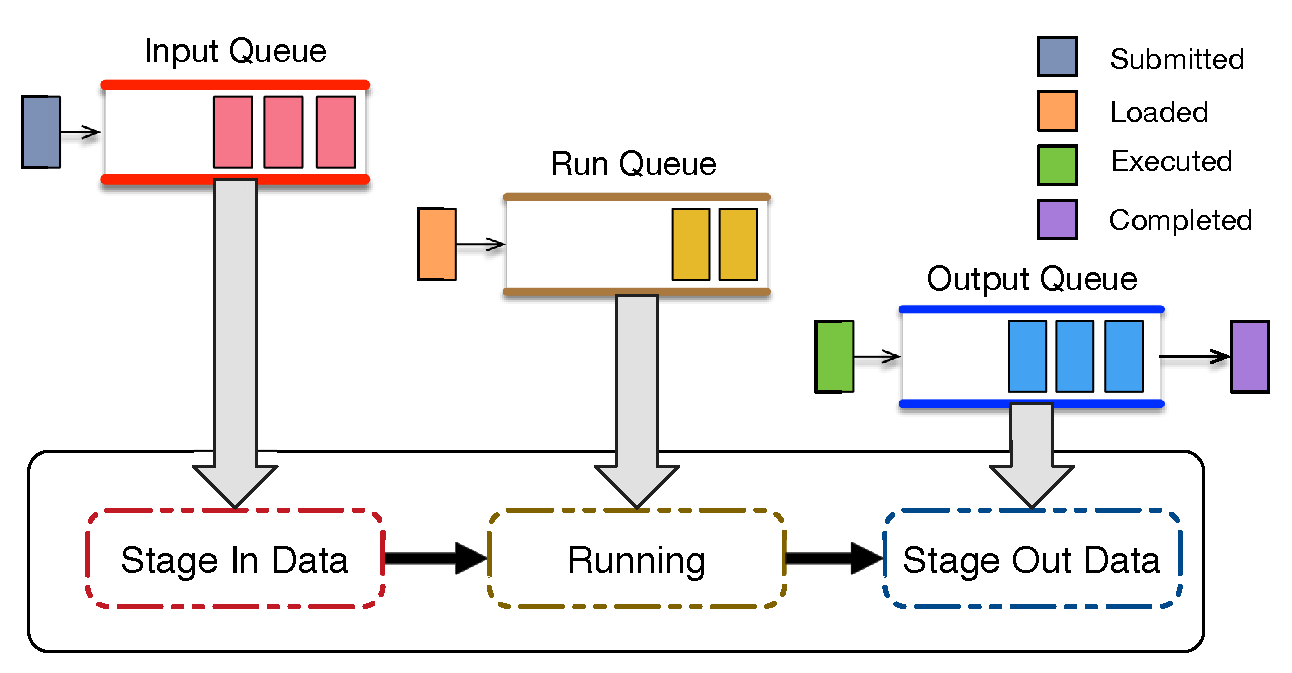
\includegraphics[width=3.6in]{CerberusQueues}
        %\caption{Scheduling Process of Burst Buffer Aware Cerberus}
        %\label{Fig:CerberusQueues}
%\end{figure}

\begin{figure}[!t]
        \centering
        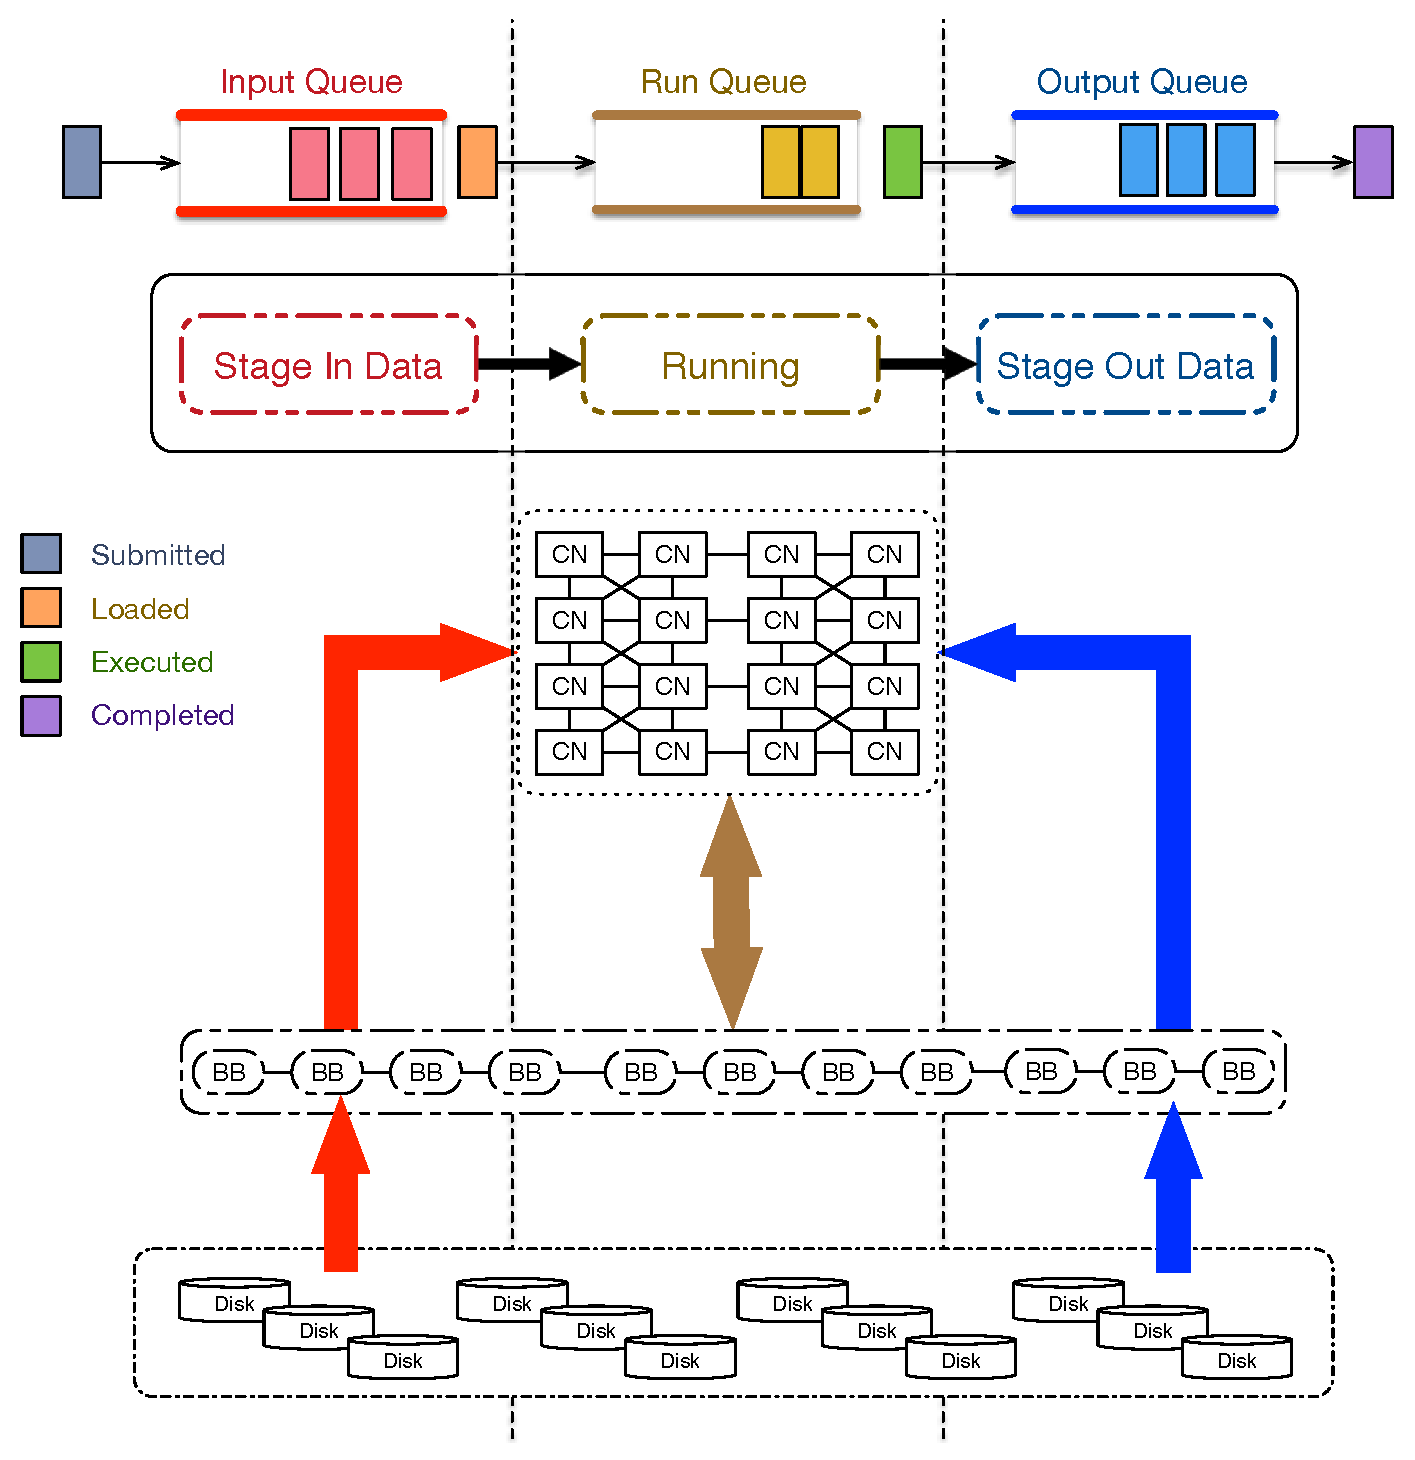
\includegraphics[width=3.6in]{CerberusBBSystem}
        \caption{Scheduling Workflow of Cerberus}
        \label{Fig:CerberusQueues}
\end{figure}


\subsection{Optimize Stage-In Phase}
In the stage-in phase, only burst buffer demand is considered.
Scheduling is made based on the value of $bb\_in$ of jobs in $Q_I$.
If we care about data transfer throughput,
we should transfer as much data as possible by doing the following optimization:
\begin{align*}
        & \max \sum_{i\in S} bb\_in_i \\
        & s.t. \sum_{i\in S} bb\_in_i \leq BB_{available} \numberthis \label{Equ:MaxTransferData}
        %\left\{
                %\begin{array}{l}
                        %S \subseteq J_{Q_I} \\ [1em]
                        %\sum_{i\in S} bb\_in_i \leq BB_{available}
                %\end{array} 
        %\right.
\end{align*}
where $J_{Q_I}$ stands for all jobs in input queue at the time considering,
$S\subseteq J_{Q_I}$ is the set of job selected by Cerberus,
$bb\_in_i$ is the burst buffer demand of $job_i$,
$BB_{available}$ is system's available amount of burst buffer.

If we care about task parallelism, following optimization could help:
\begin{align*}
        & \max |S| \\
        & s.t. \sum_{i\in S} bb\_in_i \leq BB_{available} \numberthis \label{Equ:MaxTaskNumber}  
        %\left\{
                %\begin{array}{l}
                        %S \subseteq J_{Q_I} \\ [1em] 
                        %\sum_{i\in S} bb\_in_i \leq BB_{available}
                %\end{array} 
        %\right.
\end{align*}
The number of tasks doing data loading will be maximized.


\subsection{Optimize Running Phase}
Running jobs require not only compute nodes, but burst buffer to ensure performance and correctness.
Scheduling are accordingly made based on the value of $c$ and $bb\_run$ of jobs in $Q_R$.
To maximize multiple types of resource's utilization,
we convert it to the knapsack problem by defining the value of the $job_i$ as
\begin{equation}
        v_i = \frac{c_i / CN}{rt_i} \times \frac{bb\_run_i / BB}{rt_i}
        \label{Equ:DefValue}
\end{equation}
where $rt_i$ is the running time of $job_i$, the time it takes up the computing nodes.
By defining \textit{value} as Equation~\ref{Equ:DefValue},
we prefer these tasks that claims to take up node resources with short duration.
Unfortunately, it is difficult to predict $rt_i$ before actually running the job.
Of course we could use the \textit{expected running time} $ert_i$ specified by user.
However, by examining the log traces from ANL\cite{JobTrace},
we found that the variance between $rt_i$ and $ert_i$ is significantly different.
For now we can just assume $ert_i$ represent expected running time of $job_i$.
In the future, we could adopt machine learning or data mining ideas
to predict the running time of a job with demand vector.
%Notice that then the value of a task is proportional to $c_i*bb_i$.
The optimizing formula can thus be
\begin{align*}
        & \max \sum_{i \in S}\frac{c_i}{ert_i} * \frac{bb\_run_i}{ert_i} \\
        & s.t. \left\{
                \begin{array}{l}
                        %S \subseteq J_{Q_R} \\ [1em]
                        \sum_{i \in S} c_i \leq CN_{available} \\[1em] \numberthis \label{Equ:MaxProduct} 
                        \sum_{i \in S} bb\_run_i \leq BB_{available}
                \end{array} 
        \right.
\end{align*}
where $J_{Q_R}$ is the set of jobs in running queue,
$S\subseteq J_{Q_R}$ stands for jobs selected by scheduler,
$CN_{available}$ and $BB_{available}$ represent the amount of system's available resource
(compute nodes and burst buffer) at current moment.

\subsection{Optimize Stage-Out Phase}
Scheduling are made based on the value of $bb\_out$ of jobs in $Q_O$.
Optimization formula for different purpose are almost the same as
Equation~\ref{Equ:MaxTransferData} and Equation~\ref{Equ:MaxTaskNumber}
in stage-in scheduling, except that $bb\_in$ is replaced with $bb\_out$,
$J_{Q_I}$ is replaced with $J_{Q_O}$, the job set of output queue.


\subsection{Solving the Optimization Problems}
It is trivial to show that optimization problem~\ref{Equ:MaxTransferData}
and~\ref{Equ:MaxTaskNumber}
are equivalent to 0-1 knapsack problem.
Problem~\ref{Equ:MaxProduct} can be informally treat as two dimension 0-1 knapsack problem.
In fact, we expect all of them are NP-hard problems.
We can solve them with dynamic programming in pseudo polynomial time.
Applying memorization could also help accelerate the solving process.
In fact we are not interested in the optimal result of problem~\ref{Equ:MaxTransferData},
problem~\ref{Equ:MaxTaskNumber} and problem~\ref{Equ:MaxProduct} at all
but in a combination of jobs that yields the optimal solution,
which can also be easily tracked back down by keeping memorizations.

%The solution to Problem~\ref{Equ:MaxTransferData},
%Problem~\ref{Equ:MaxTaskNumber} and Problem~\ref{Equ:MaxProduct} are similar.
First, for Problem~\ref{Equ:MaxTransferData}, the recursive relationship is
given by Recursion~\ref{Equ:MaxTransferDataRecursion}.
In~\ref{Equ:MaxTransferDataRecursion}, the memo we keeps during solving is
the optimal solution for 
$jobs=(job_1, job_2, \ldots, job_i)$ with $w$ GB of available burst buffer.
It turns out that the recursion for Problem~\ref{Equ:MaxTaskNumber} is
extremely similar to~\ref{Equ:MaxTransferDataRecursion}
The memo in Recursion~\ref{Equ:MaxTaskNumberRecursion} is the same
as that in Recursion~\ref{Equ:MaxTransferDataRecursion}.
The recursion for Problem~\ref{Equ:MaxProduct} is a little bit complicated.
Here we should keep the memo of the optimal solution for $jobs=(job_1, job_2, \ldots, job_i)$
with $c$ computing nodes and $w$ GB of burst buffer being available.

Scheduler can obtain an optimal combination of jobs by examining the memo.
Take the problem~\ref{Equ:MaxProduct} problem for example.
We start from $dp(n, CN, BB)$.
If $c_n \leq CN$ and $bb\_in_n \leq BB$, $job_n$ should be scheduled if
$dp(i-1, c, w) \leq dp(i-1, c - c_i, w - bb\_in_i) + c_i bb\_in_i$ and
recurse with $dp(n - 1, CN - c_i, BB - bb\_in_i)$;
otherwise, $job_n$ should be skipped and we recurse the process on $dp(n-1, CN, BB)$.
The time complexity of solving Equation~\ref{Equ:MaxTransferDataRecursion} and
Equation~\ref{Equ:MaxTaskNumberRecursion} is $O(n\times BB)$.
The time complexity of solving Recursion~\ref{Equ:MaxProductRecursion}
is $O(n\times CN\times BB)$.
Notice that $CN$ and $BB$ may be very large integers,
making the pseudo-polynomial algorithm unsuitable
to be used online by scheduler.
In practice, we could reduce the time complexity by allocating resource
in a coarser granularity.
For example, jobs usually asks for compute node in the unit of $cn\_unit = 512$ nodes;
their demands for burst buffer nodes are usually in the unit of $bb\_unit = 100$ GB.
We can divide both $CN$ and $c_i$ by $cn\_unit$;
divide both $BB$ and $bb\_in, bb\_run, bb\_out$ by $bb\_unit$.
It is also possible to reduce the value of $n$, the number of jobs in the queue.
For example, we can consider only $\frac{1}{\alpha}n$ jobs in the queue.
This will give us only the partial optimal solution
in exchange of less computation complexity.

\begin{strip}
        \begin{align}
                dp(i, w) = & 
                \left\{
                        \begin{array}{l}
                                0, \text{ if $i=0$ } \\ [0.4em]
                                dp(i-1, w), \text{ if $bb\_in_i > w$} \\ [0.4em]
                                \max \{ dp(i-1, w), dp(i-1, w-bb\_in_i) + bb\_in_i \}, \text{ if $bb\_in_i \leq w$}
                        \end{array} 
                \right.
                \label{Equ:MaxTransferDataRecursion} 
        \end{align}
\end{strip}
\begin{strip}
        \begin{align}
                dp(i, w) = &
                \left\{
                        \begin{array}{l}
                                0, \text{ if $i=0$ } \\ [0.4em]
                                dp(i-1, w), \text{ if $bb\_in_i > w$} \\ [0.4em]
                                \max \{ dp(i-1, w), dp(i-1, w-bb\_in_i) + 1 \}, \text{ if $bb\_in_i \leq w$}
                        \end{array} 
                \right.
                \label{Equ:MaxTaskNumberRecursion}
        \end{align}
\end{strip}
\begin{strip}
        \begin{align}
                dp(i, c, w) = &
                \left\{
                        \begin{array}{l}
                                0, \text{ if $i=0$ } \\ [0.4em]
                                dp(i-1, c, w), \text{ if $c_i > c$ or $bb\_run_i > w$} \\ [0.4em]
                                \max \{ dp(i-1, c, w), dp(i-1, c - c_i, w - bb\_run_i) + v_i \}, \text{ if $c_i \leq c$ and $bb\_run_i \leq w$}
                        \end{array} 
                \right.
                \label{Equ:MaxProductRecursion}
        \end{align}
\end{strip}



\section{Simulation Results}
We consider simulating the full Trinity super computer.
The number of compute nodes on Trinity is about 18936, 9436 Intel Haswell nodes
and at least 9500 Intel Xeon Phi nodes.
There are 16 cores on each processor, thus totally 302976 cores.
In the following experiments, we compare two identical system except that
IO nodes are replaced by the same number of burst buffer nodes.
Eventually Trinity plans to delivery up to 576 burst buffer nodes of 3.7 PB,
consisted of Trinity IO nodes with PCIe SSD card.
They are globally accessible and distributed among cabinets.
According to their hardware design, in our simulation, 
Burst buffer nodes provide total capacity of 4.0 PB PCIe SSD intermediate storage.
Sequential read/write between burst buffer and compute nodes is 8.0 GB/s.
Bandwidth between CPU node and IO node is set to 2.5 GB/s.
Job trace is from ANL's Blue Gene Intrepid system from January to September 2009.
Each log entry contains information like jobs' submission time, running time,
number of cores user requested and so on. 
It is truncated so that only the first 1185 jobs are used in simulation.
We patched 3 fields to each job's log entry: the amount of input data $data\_in$,
the amount of written data during checkpointing $data\_run$ and the amount of output data $data\_out$.
We assume they follows uniform distribution with low boundary 1 TB and high boundary 60 TB.
The patches 3 fields may or may not be used in scheduling,
depends on both the model of the jobs and the experiment scenario.

Following sections discuss or answer 3 key questions.
Will Cerberus improve application performance by utilizing burst buffer nodes?
Can Cerberus with optimization improve application performance?
Will job demand on burst buffer effect Cerberus?

\subsection{Cerberus vs. 1-Phase Batch Scheduler}
\label{Sec:Sim:DirectIOvsBB}
In this section, we demonstrate that by utilizing burst buffer nodes,
job scheduler could improve the applications' performance.
Figure \ref{Fig:DirectIOvsBBResponseTime} compares CDF of the response time of 1000 jobs.
When scheduler can allocate burst buffer to jobs (denoted as Plain BB),
all jobs finish in 360,000 seconds counting from their submission time.
However, the worst case in system without burst buffer (denoted as Direct IO) is catastrophical.
There are jobs that takes almost 1,400,000 seconds to finish,
almost as 4 times slow as the most non-responsive job in system equipped with burst buffer.
In average case, more than 90\% of the jobs scheduled by Cerberus response faster than 1-Phase Batch scheduler.
The improvement mainly comes from the difference of IO operation efficiency between
traditional IO nodes and burst buffer nodes.
There are only less than 10\% of the jobs response quicker without needing burst buffer.

Using the collected completion time, we can calculate system's throughput over time sequence.
Figure \ref{Fig:DirectIOvsBBThroughput} shows the number of tasks finished
in a fixed time unit (500 seconds) for system using burst buffer nodes and not.
It takes more than 1,382,769 seconds for the system without burst buffer nodes to
server all 1000 jobs.
The last job is job \#1150, which requested 4096 cores and 49 TB data space.
It starts at 1169 seconds and finishes at 1,383,938 seconds.
In contrast, when system installed burst buffer nodes,
it accomplish the same 1185 jobs in 336,396 seconds.
Job \#1150 is the second last job finished, but both its completion time and response time
are significantly reduced, 268701 and 267531 seconds respectively.
As indicated by the horizontal lines (green for Direct IO and yellow for Plain BB),
the ratio of average throughput between two systems is about 4, namely 1.769 to 0.431.
This approximately coincides with the response speedup due to burst buffer equipments.


\begin{figure}[!t]
\centering
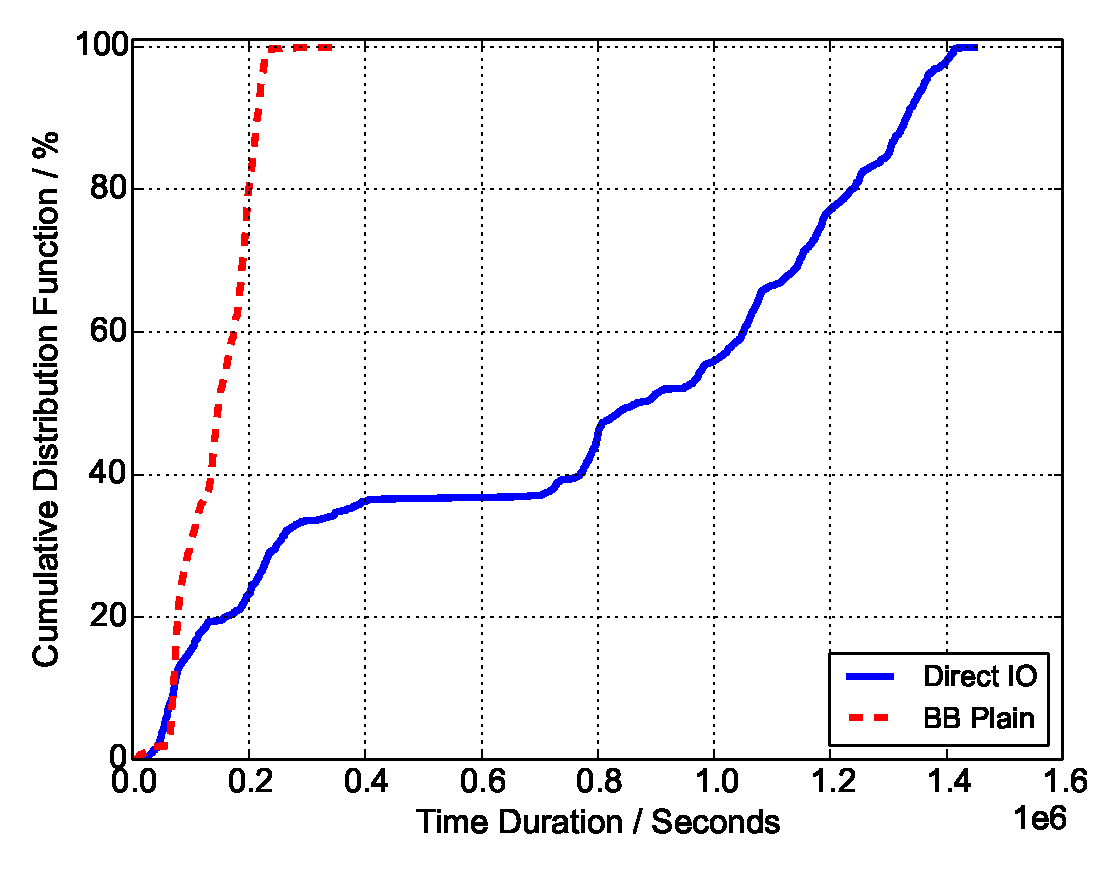
\includegraphics[width=3.2in]{DrawDirectIOvsBB/1000jobs_direct_vs_bb_response}
\caption{Application Response Time, IO Node Only vs. Burst Buffer System}
\label{Fig:DirectIOvsBBResponse}
\end{figure}

\begin{figure}[!t]
\centering
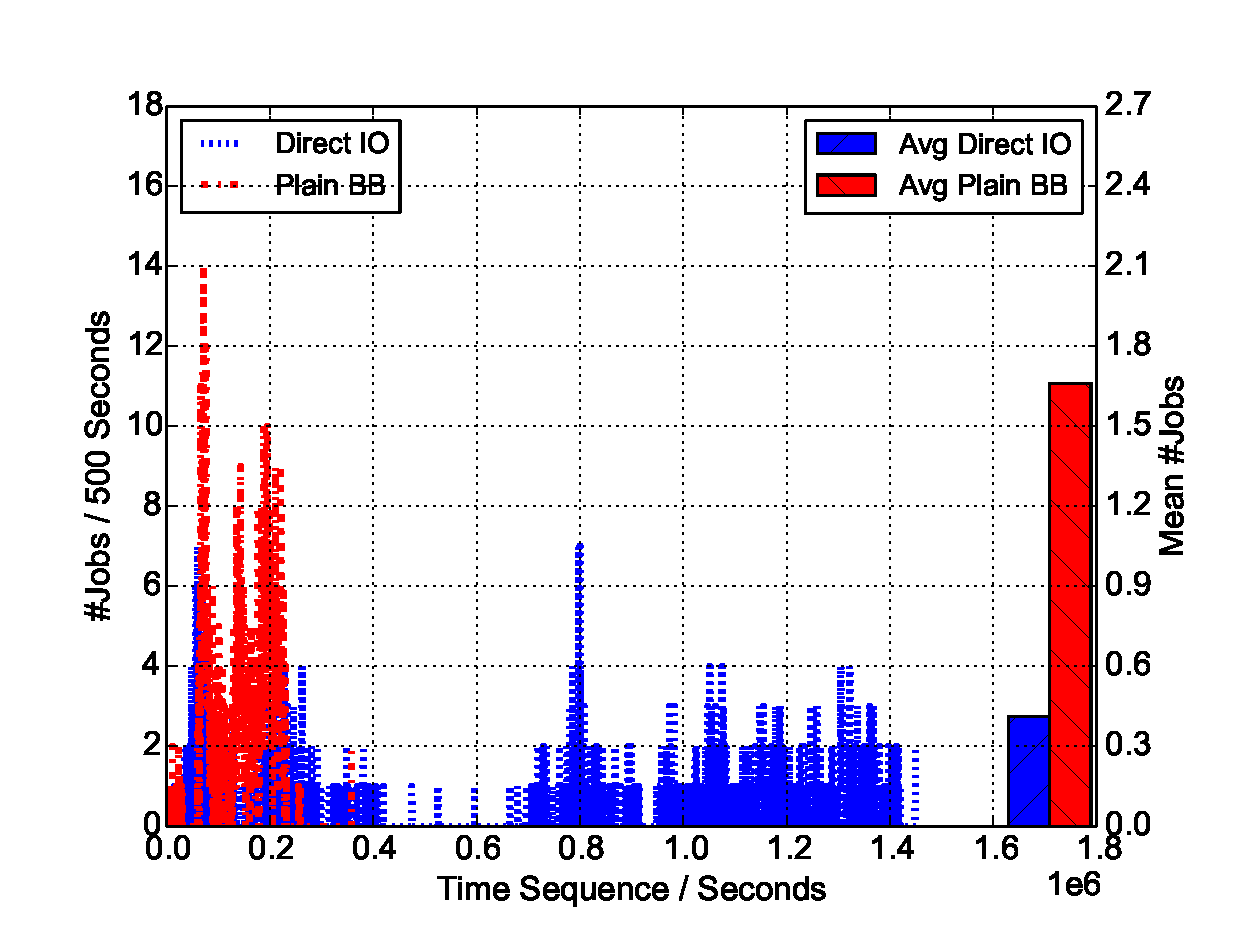
\includegraphics[width=3.2in]{DrawDirectIOvsBB/1000jobs_direct_vs_bb_throughput}
\caption{Application Throughput, IO Node Only vs. Burst Buffer System}
\label{Fig:DirectIOvsBBThroughput}
\end{figure}


\subsection{Cerberus vs. Cerberus with Optimization}
If we consider optimizing either burst buffer's data throughput or the parallelism across jobs,
dynamic programming based job scheduler can further reduce jobs' wait time.
We plot in Figure \ref{Fig:DPvsFIFOResponse} the resulting response time of three different scheduler
regarding how they handle jobs in their queues(input queue, run queue, and output queue).
The first scheduler uses naive first come first serve (FCFS) policy.
Whoever at the front of queue are considered favorably.
The second and third scheduler treat jobs in run queue identically.
They choose jobs according to the optimization solution given by \ref{Equ:MaxProductRecursion}
However, they treat jobs in the input queue and output queue differently.
The second scheduler will select these jobs in its queue so that volume of transferred data is maximized.
The third scheduler tries to optimize the number of schedulable jobs by using \ref{Equ:MaxTaskNumberRecursion}.


\begin{figure}[!t]
\centering
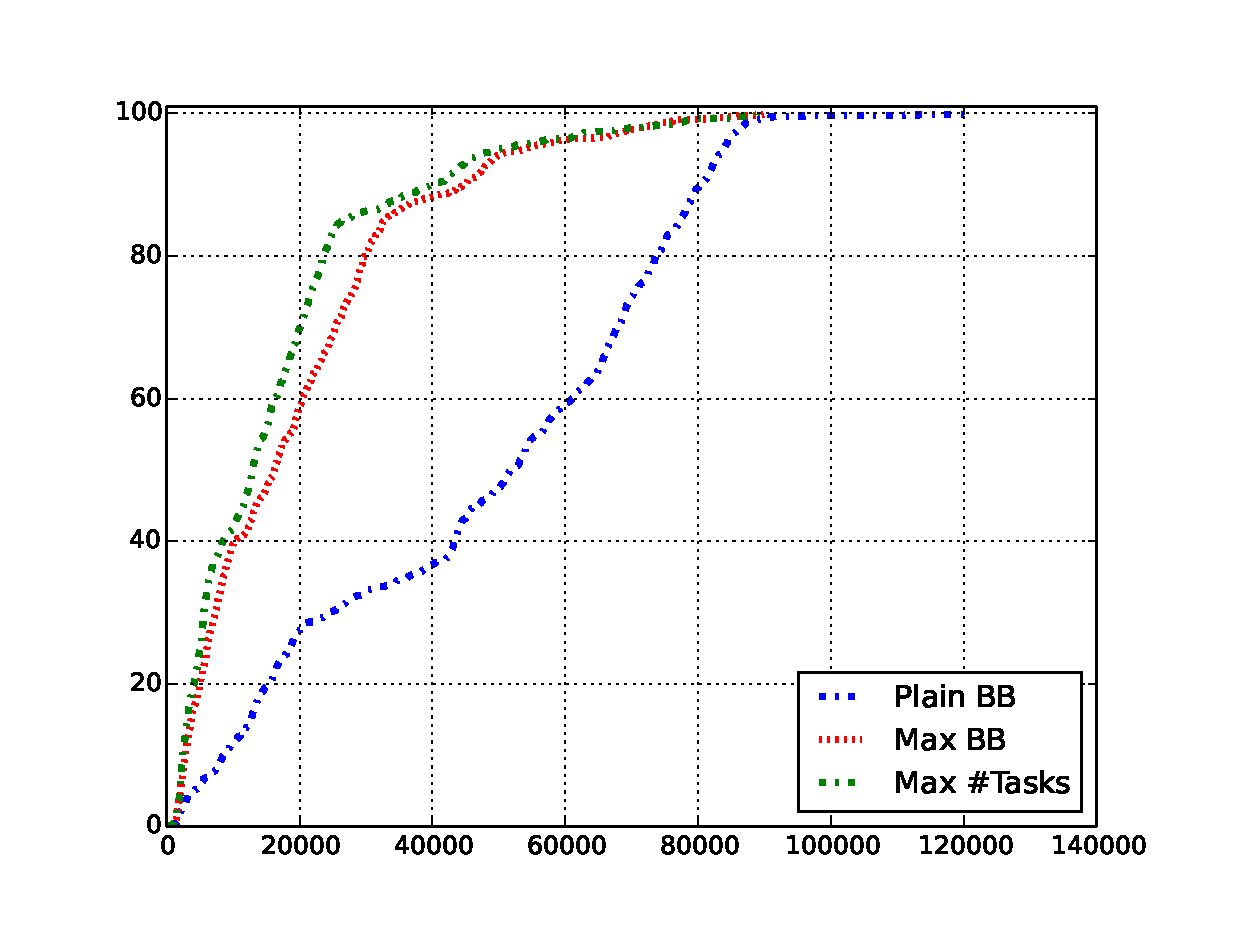
\includegraphics[width=3.2in]{DrawDPvsFIFO/1000jobs_dp_vs_fifo_response}
\caption{Application Response, Dynamic Programming vs. FCFS}
\label{Fig:DPvsFIFOResponse}
\end{figure}


\begin{figure}[!t]
\centering
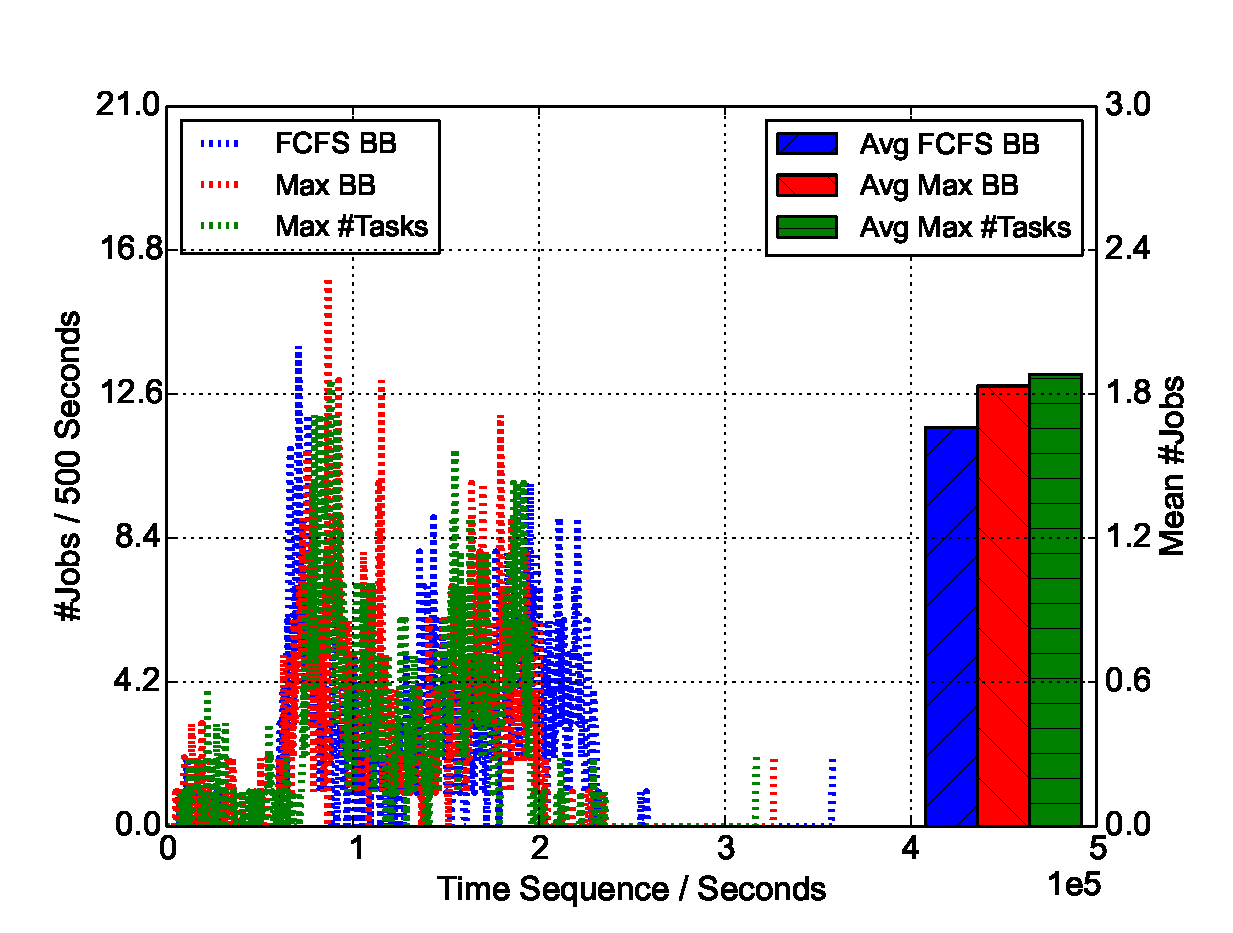
\includegraphics[width=3.2in]{DrawDPvsFIFO/1000jobs_dp_vs_fifo_throughput}
\caption{Application Throughput, Dynamic Programming vs. FCFS}
\label{Fig:DPvsFIFOThroughput}
\end{figure}


\subsection{Cerberus vs. Demand Granularity}
In this section we validate our 3-phase model.
Applications are benefited when scheduler dividing jobs into 3 separated phases and 
scheduling are based on corresponding burst buffer demand in each phase.
This suggests that user should provide burst buffer demand as granular as possible.

In Figure \ref{Fig:3Pvs1PResponseTime}, we plot 3 different scheduling results by 3 FCFS scheduler.
Jobs in the first case, denoted as Direct BB, are modeled as just 1 phase because user just provides
a general burst buffer demand throughout entire application life time.
We assume this demand is the $\max \{data\_in, data\_out, data\_run\}$.
This is the traditional scheduling scheme except job has additional
burst buffer demand and scheduler must subject to burst buffer capacity constraint.
Jobs in the second and third cases have 3 phases and are scheduled by Cerberus.
However, in the second case, denoted as Plain BB 1D, Cerberus only knows the overall burst buffer demand,
same as the information in case 1.
In the 3rd case, named Plain BB 3P, users kindly provided all the burst buffer demand in all 3 phases.
This is the same case as in section \ref{Sec:Sim:DirectIOvsBB} when we demonstrating burst buffer is beneficial.
We simulate the 3 cases with the same generated random data volume.
For 1-phase-modeled jobs, scheduler will make decision based on $\max \{data\_in, data\_out, data\_run\}$
since we assume user will only tell the upper bound of its application's demand.
However, in simulation, we use the generated data amount as the same as 3-modeled jobs.
%Response time of system without burst buffer devices are also plotted for comparison.

Unsurprisingly, jobs' response time is improving as long as they could utilizing burst buffer.
Let's compare scheduling results of 1-phase and 3-phase, both of which only have rough data information of application.
More than 60\% of the 3-phase-modeled jobs finish faster than 1-phase-modeled jobs.
The longest 3-phase-modeled job takes 400,000 seconds to finish while the slowest 1-phase-modeled job
needs about 540,000 seconds to finish.
The improvement is about 26\% for the worst case.
The reason of such improvement is as follows.
For the 1-phase-modeled jobs, burst buffer nodes will be exclusively taken by scheduled jobs
throughout their lifetime.
In contrast, each time a 3-phase-modeled job finish inputing, running or outputing,
Cerberus will reclaim burst buffer and CPU resources.
This gives Cerberus more opportunity to schedule the system resources.
At last, when comparing the case of 3-phase IRO with 3-phase D, we find another advantage of our 3-phase model.
If benign users can provide finer-grain information of data/IO demand,
Cerberus can programme each queue separately and get better scheduling result.
In our simulation, when Cerberus knows more about application's demand in different phases,
the worst absolute response time is less than 300,000 seconds.
This is 25\% improvement to 3-phase-modeled jobs when Cerberus only knows the upper bound of data demand,
44\% better than the slowest 1-phase-modeled job.
In average case, 80\% of the 3-phase-modeled jobs scheduled by Cerberus finish earlier than 1-phase-modeled jobs,
on the same condition that the same amount of burst buffer nodes are available to applications.
Meanwhile, more than 90\% of the jobs takes less time if user specifies data usage demand
at each phase to Cerberus.

Figure \ref{Fig:3Pvs1PThroughput} describes system throughput of these three different scenarios.
It helps us examine the performance of the scheduling in time sequence.
For 1-phase-modeled job, we can see an obvious 'throughput gap'
from 150,000 second to 250,000 second approximately.
This is the result of too aggressive scheduling at the beginning.
For the case of 3-phase D, throughput also starts provocatively,
but not as provocatively as 1-phase scheduling case;
it is then calmed due to frequent resource release,
indicated by multiple crests and troughs from 0 to 350,000 seconds.
The 3-phase IRO runs counter to the both previous cases.
Even though beginning with throughput trough,
Cerberus manages to make the system having high throughput from 50,000 to 250,000 seconds,
during which system can achieve throughput around 10 to 12 per 500 seconds. 
In average, the throughput of 3-phase IRO case is 1.670 jobs / 500 seconds.
It is 51.82\% higher than the Direct BB case (1.101 jobs / 500 seconds) and
17.69\% higher than the Plain BB 1D case (1.419 jobs / 500 seconds).
We believe this validates the indispensable 3 phase job model and
the necessity that user provides data capacity demand for each phase.


\begin{figure}[!t]
\centering
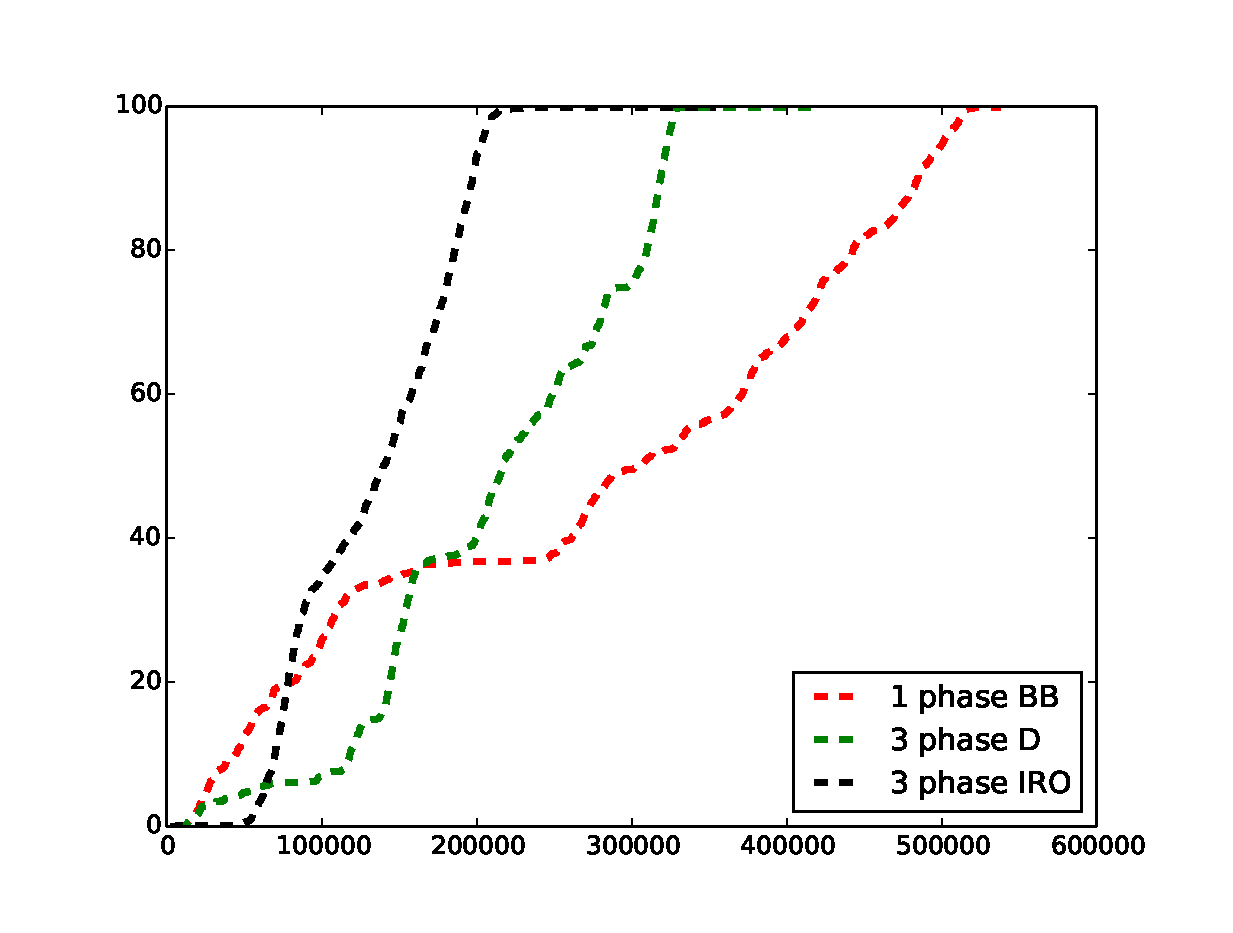
\includegraphics[width=3.2in]{Draw3Pvs1P/1000jobs_3p_vs_1p_response}
\caption{Application Response Time, 1 Phase Model vs. 3 Phase Model}
\label{Fig:3Pvs1PResponse}
\end{figure}

\begin{figure*}[!t]
\centering
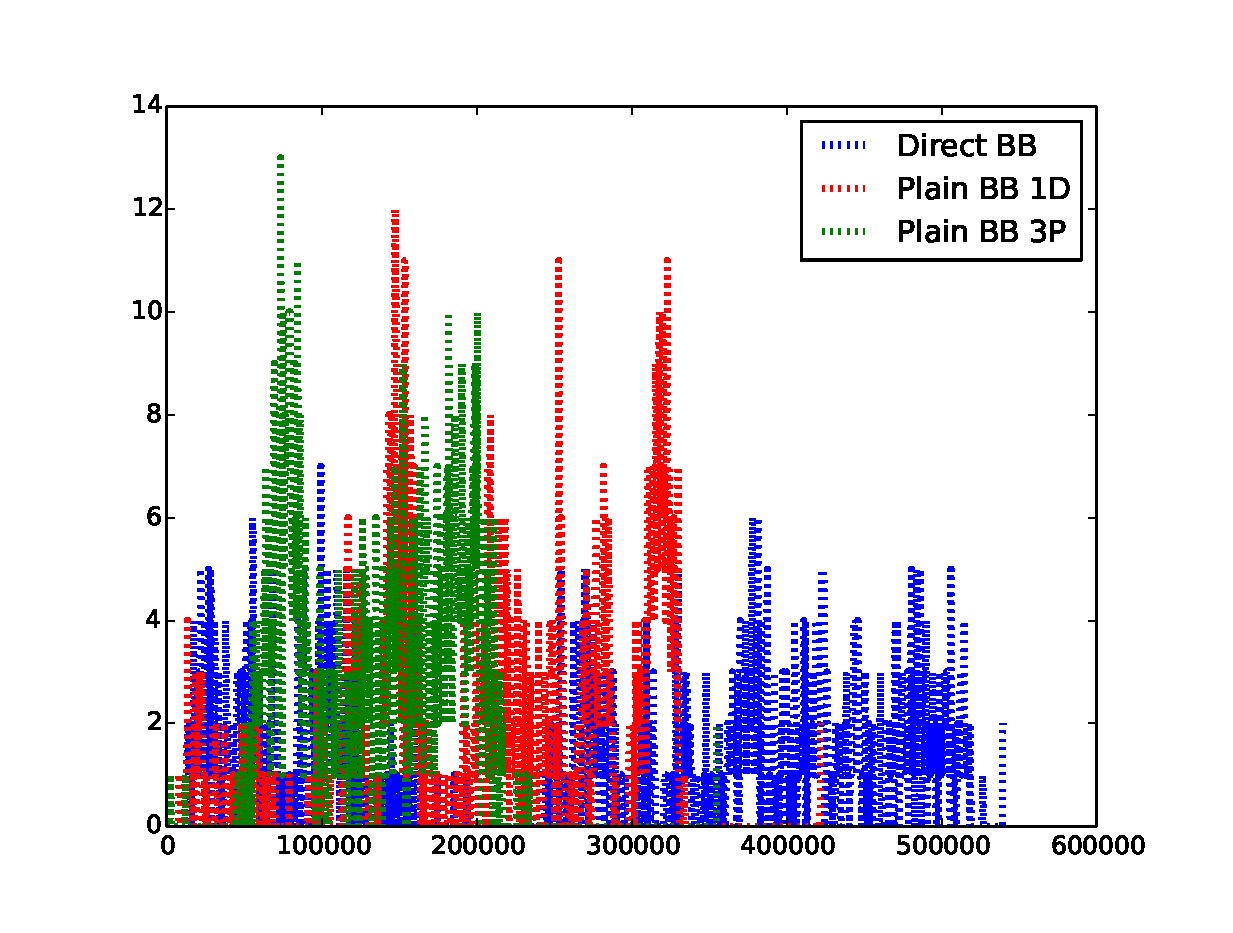
\includegraphics[width=7.0in]{Draw3Pvs1P/1000jobs_3p_vs_1p_throughput}
\caption{System Throughput, 1 Phase Model vs. 3 Phase Model}
\label{Fig:3Pvs1PThroughput}
\end{figure*}





% An example of a floating figure using the graphicx package.
% Note that \label must occur AFTER (or within) \caption.
% For figures, \caption should occur after the \includegraphics.
% Note that IEEEtran v1.7 and later has special internal code that
% is designed to preserve the operation of \label within \caption
% even when the captionsoff option is in effect. However, because
% of issues like this, it may be the safest practice to put all your
% \label just after \caption rather than within \caption{}.
%
% Reminder: the "draftcls" or "draftclsnofoot", not "draft", class
% option should be used if it is desired that the figures are to be
% displayed while in draft mode.
%
%\begin{figure}[!t]
%\centering
%\includegraphics[width=2.5in]{myfigure}
% where an .eps filename suffix will be assumed under latex, 
% and a .pdf suffix will be assumed for pdflatex; or what has been declared
% via \DeclareGraphicsExtensions.
%\caption{Simulation results for the network.}
%\label{fig_sim}
%\end{figure}

% Note that the IEEE typically puts floats only at the top, even when this
% results in a large percentage of a column being occupied by floats.


% An example of a double column floating figure using two subfigures.
% (The subfig.sty package must be loaded for this to work.)
% The subfigure \label commands are set within each subfloat command,
% and the \label for the overall figure must come after \caption.
% \hfil is used as a separator to get equal spacing.
% Watch out that the combined width of all the subfigures on a 
% line do not exceed the text width or a line break will occur.
%
%\begin{figure*}[!t]
%\centering
%\subfloat[Case I]{\includegraphics[width=2.5in]{box}%
%\label{fig_first_case}}
%\hfil
%\subfloat[Case II]{\includegraphics[width=2.5in]{box}%
%\label{fig_second_case}}
%\caption{Simulation results for the network.}
%\label{fig_sim}
%\end{figure*}
%
% Note that often IEEE papers with subfigures do not employ subfigure
% captions (using the optional argument to \subfloat[]), but instead will
% reference/describe all of them (a), (b), etc., within the main caption.
% Be aware that for subfig.sty to generate the (a), (b), etc., subfigure
% labels, the optional argument to \subfloat must be present. If a
% subcaption is not desired, just leave its contents blank,
% e.g., \subfloat[].


% An example of a floating table. Note that, for IEEE style tables, the
% \caption command should come BEFORE the table and, given that table
% captions serve much like titles, are usually capitalized except for words
% such as a, an, and, as, at, but, by, for, in, nor, of, on, or, the, to
% and up, which are usually not capitalized unless they are the first or
% last word of the caption. Table text will default to \footnotesize as
% the IEEE normally uses this smaller font for tables.
% The \label must come after \caption as always.
%
%\begin{table}[!t]
%% increase table row spacing, adjust to taste
%\renewcommand{\arraystretch}{1.3}
% if using array.sty, it might be a good idea to tweak the value of
% \extrarowheight as needed to properly center the text within the cells
%\caption{An Example of a Table}
%\label{table_example}
%\centering
%% Some packages, such as MDW tools, offer better commands for making tables
%% than the plain LaTeX2e tabular which is used here.
%\begin{tabular}{|c||c|}
%\hline
%One & Two\\
%\hline
%Three & Four\\
%\hline
%\end{tabular}
%\end{table}


% Note that the IEEE does not put floats in the very first column
% - or typically anywhere on the first page for that matter. Also,
% in-text middle ("here") positioning is typically not used, but it
% is allowed and encouraged for Computer Society conferences (but
% not Computer Society journals). Most IEEE journals/conferences use
% top floats exclusively. 
% Note that, LaTeX2e, unlike IEEE journals/conferences, places
% footnotes above bottom floats. This can be corrected via the
% \fnbelowfloat command of the stfloats package.




\section{Conclusion}
The conclusion goes here.




% conference papers do not normally have an appendix



% use section* for acknowledgment
\ifCLASSOPTIONcompsoc
  % The Computer Society usually uses the plural form
  \section*{Acknowledgments}
\else
  % regular IEEE prefers the singular form
  \section*{Acknowledgment}
\fi


The authors would like to thank...





% trigger a \newpage just before the given reference
% number - used to balance the columns on the last page
% adjust value as needed - may need to be readjusted if
% the document is modified later
%\IEEEtriggeratref{8}
% The "triggered" command can be changed if desired:
%\IEEEtriggercmd{\enlargethispage{-5in}}

% references section

% can use a bibliography generated by BibTeX as a .bbl file
% BibTeX documentation can be easily obtained at:
% http://mirror.ctan.org/biblio/bibtex/contrib/doc/
% The IEEEtran BibTeX style support page is at:
% http://www.michaelshell.org/tex/ieeetran/bibtex/
%\bibliographystyle{IEEEtran}
% argument is your BibTeX string definitions and bibliography database(s)
%\bibliography{IEEEabrv,../bib/paper}
%
% <OR> manually copy in the resultant .bbl file
% set second argument of \begin to the number of references
% (used to reserve space for the reference number labels box)
\begin{thebibliography}{1}

\bibitem{IEEEhowto:kopka}
H.~Kopka and P.~W. Daly, \emph{A Guide to \LaTeX}, 3rd~ed.\hskip 1em plus
  0.5em minus 0.4em\relax Harlow, England: Addison-Wesley, 1999.

\end{thebibliography}




% that's all folks
\end{document}


